\documentclass[main.tex]{subfiles}
\begin{document}
Fondamentalement il n'y a pas de différence entre une modulation analogique et une modulation numérique.
\begin{rem}
  Le cours de modulation analogique (AM,FM, bande de Carson ...) a été traité dans l'UE 431.
\end{rem}
\paragraph{Notation}:
\begin{itemize}
\item $u(t)$ est le signal modulant.
\item $p(t)$ est la porteuse.
\item $s(t)$ est le signal de sortie, modulé.
\end{itemize}

\section{Modulation numérique}
\begin{defin}
  La modulation numérique est une modulation analogique dont le modulant est un signal type codé en bande de base.
\end{defin}
\begin{prop}
  On se donne différetent indicateur de la qualité de la modulation/transmission:
  \begin{itemize}
  \item L'efficacité spectrale:
    \[
      \eta = \frac{D}{B} ,\text{ avec } D = R.\log_2(M) \text{ débit binaire  et } B \text{ Bande occupée}
    \]
  \item L'énergie bit sur la puissance de bruit:
    \[
      \frac{E_b}{N_0} = \frac{\text{Energie bit} (J/bit)}{\text{DSP de bruit unilatéral} (W/Hz)}
    \]
  \item Le rapport signal à Bruit:
    \[
      RSB = \frac{P_s}{P_b} = \frac{DE_b}{BN_0} = \eta \times \frac{E_b}{N_0}
    \]
  \end{itemize}
\end{prop}
\section{Modulation d'amplitude}
On parle de modulation ASK (Amplitude shift Keying).
Le signal $u(t)$ prend $M$ valerus discrète (pour une transmission $M-aire$).
\begin{prop}
  \begin{itemize}
  \item Pour $u(t)$ NRZ, unipolaire à $M$ niveaux et impulsion rectangulaire on
    a:
  \[
    B_{ASK-rect} = 2R = \frac{2}{T}
  \]
\item Si $u(t)$ est constitué d'impulsion de Nyquist:
  \[
    B_{ASK-N} = 2R = \frac{2}{2T} =\frac{1}{T}
  \]
\end{itemize}
\end{prop}
\begin{rem}
 Cette modulation ne dépend pas de la fréquence de la porteuse (ni de sa phase), mais est strès sensible au bruit additif (fadding).
\end{rem}
\begin{exemple}
{Modulation OOK}
Pour un signal binaire on peux réaliser une modulation tout ou rien:
  \begin{figure}[H]
    \centering
    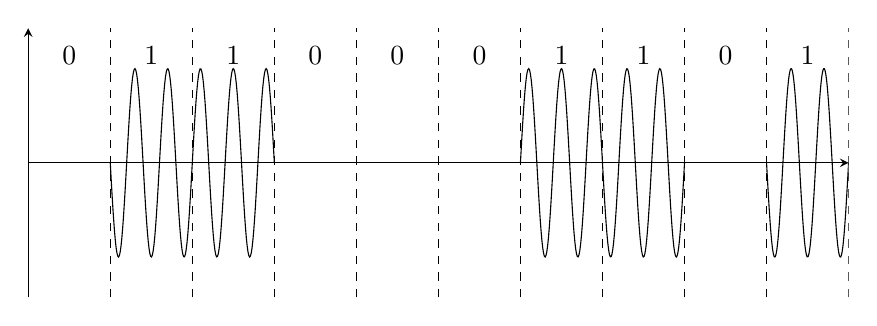
\begin{tikzpicture}
        \begin{axis}
          [axis lines = middle,height=5cm, width=12cm,
          xmin=0,xmax=450,ymin=-1,ymax=1,
          domain=0:360,samples=200, xtick=\empty,ytick=\empty]
          \addplot[black,domain=45:135]{0.7*sin(20*x)};
          \addplot[black,domain=270:360]{0.7*sin(20*x)};
          \addplot[black,domain=405:450]{0.7*sin(20*x)};
          \pgfplotsinvokeforeach{1,...,12}{%
          \draw[dashed] (axis cs:45*#1,-1) -- (axis cs:45*#1,1);}
          \node at (axis cs: 0+22.5,0.8){0};
          \node at (axis cs: 45+22.5,0.8){1};
          \node at (axis cs: 90+22.5,0.8){1};
          \node at (axis cs: 135+22.5,0.8){0};
          \node at (axis cs: 180+22.5,0.8){0};
          \node at (axis cs: 225+22.5,0.8){0};
          \node at (axis cs: 270+22.5,0.8){1};
          \node at (axis cs: 315+22.5,0.8){1};
          \node at (axis cs: 360+22.5,0.8){0};
          \node at (axis cs: 405+22.5,0.8){1};
       \end{axis}
    \end{tikzpicture}
    \caption{modulation OOK}
  \end{figure}
  On alors l'efficacité spectrale:
  \[
    \eta_{rect}  = \frac{D}{B} = 0.5 bit/s/Hz
  \]
  \[
    \eta_{N} = \frac{D}{B} = 1 bit/s/Hz
  \]
\end{exemple}
\section{Modulation angulaires}
\begin{prop}
  Dans le cas des modulation PSK :
  \begin{itemize}
  \item L'amplitude est constante
  \item seule $\Phi(t)$ code l'information numérique:
    \[
      s(t) = \Re\left[u.exp(j2\pi f_0 t+ \Phi(t))\right] = \Re\left[\underline{u}.exp(j2\pi f_0t)\right]\]
    
  \end{itemize}
\end{prop}
\begin{exemple}
  Dans le cas d'une modulation BPSK: $\Phi(t) = 0 \text{ ou }\pi $ à  la fréquence $R =\frac{1}{T_b}$ on a en en fait une modulation d'amplitude:
   \[
     s(t) = \pm A.\cos(\omega_0 t+\phi)
   \]
   C'est une modulation d'amplitude par un modulant NRZ antipolaire. $B_{BPSK-rect} = 2R$.
   
\end{exemple}
\section{FSK cohérente}
\section{FSK incohérente}
\section{Démodulation}

\section{Modulation dérivées}
\section{MAQ}
\section{Exemple d'application}






\end{document}


%%% Local Variables:
%%% mode: latex
%%% TeX-master: "main"
%%% End:
